\chapter{Anhang}

\section{Verwendete Hilfsmittel}
In der Tabelle \ref{tab:tooling} sind die im Rahmen der Bearbeitung des Themas der \IthesisKindDE~verwendeten Werkzeuge und Hilfsmittel aufgelistet.

\begin{table}[h!] %TODO: ausfüllen
\caption{Verwendete Hilfsmittel und Werkzeuge}
\begin{tabular}{|l|l|}
\hline 
\rowcolor{lightgray} Tool & Verwendung \\
\hline
\LaTeX & Textsatz- und Layout-Werkzeug verwendet zur Erstellung dieses Dokuments \\
\hline
 & \\
\hline
\end{tabular}
\label{tab:tooling}
\end{table}

\section{Abbildungen}

\begin{figure}[htbp]
    \begin{center}
        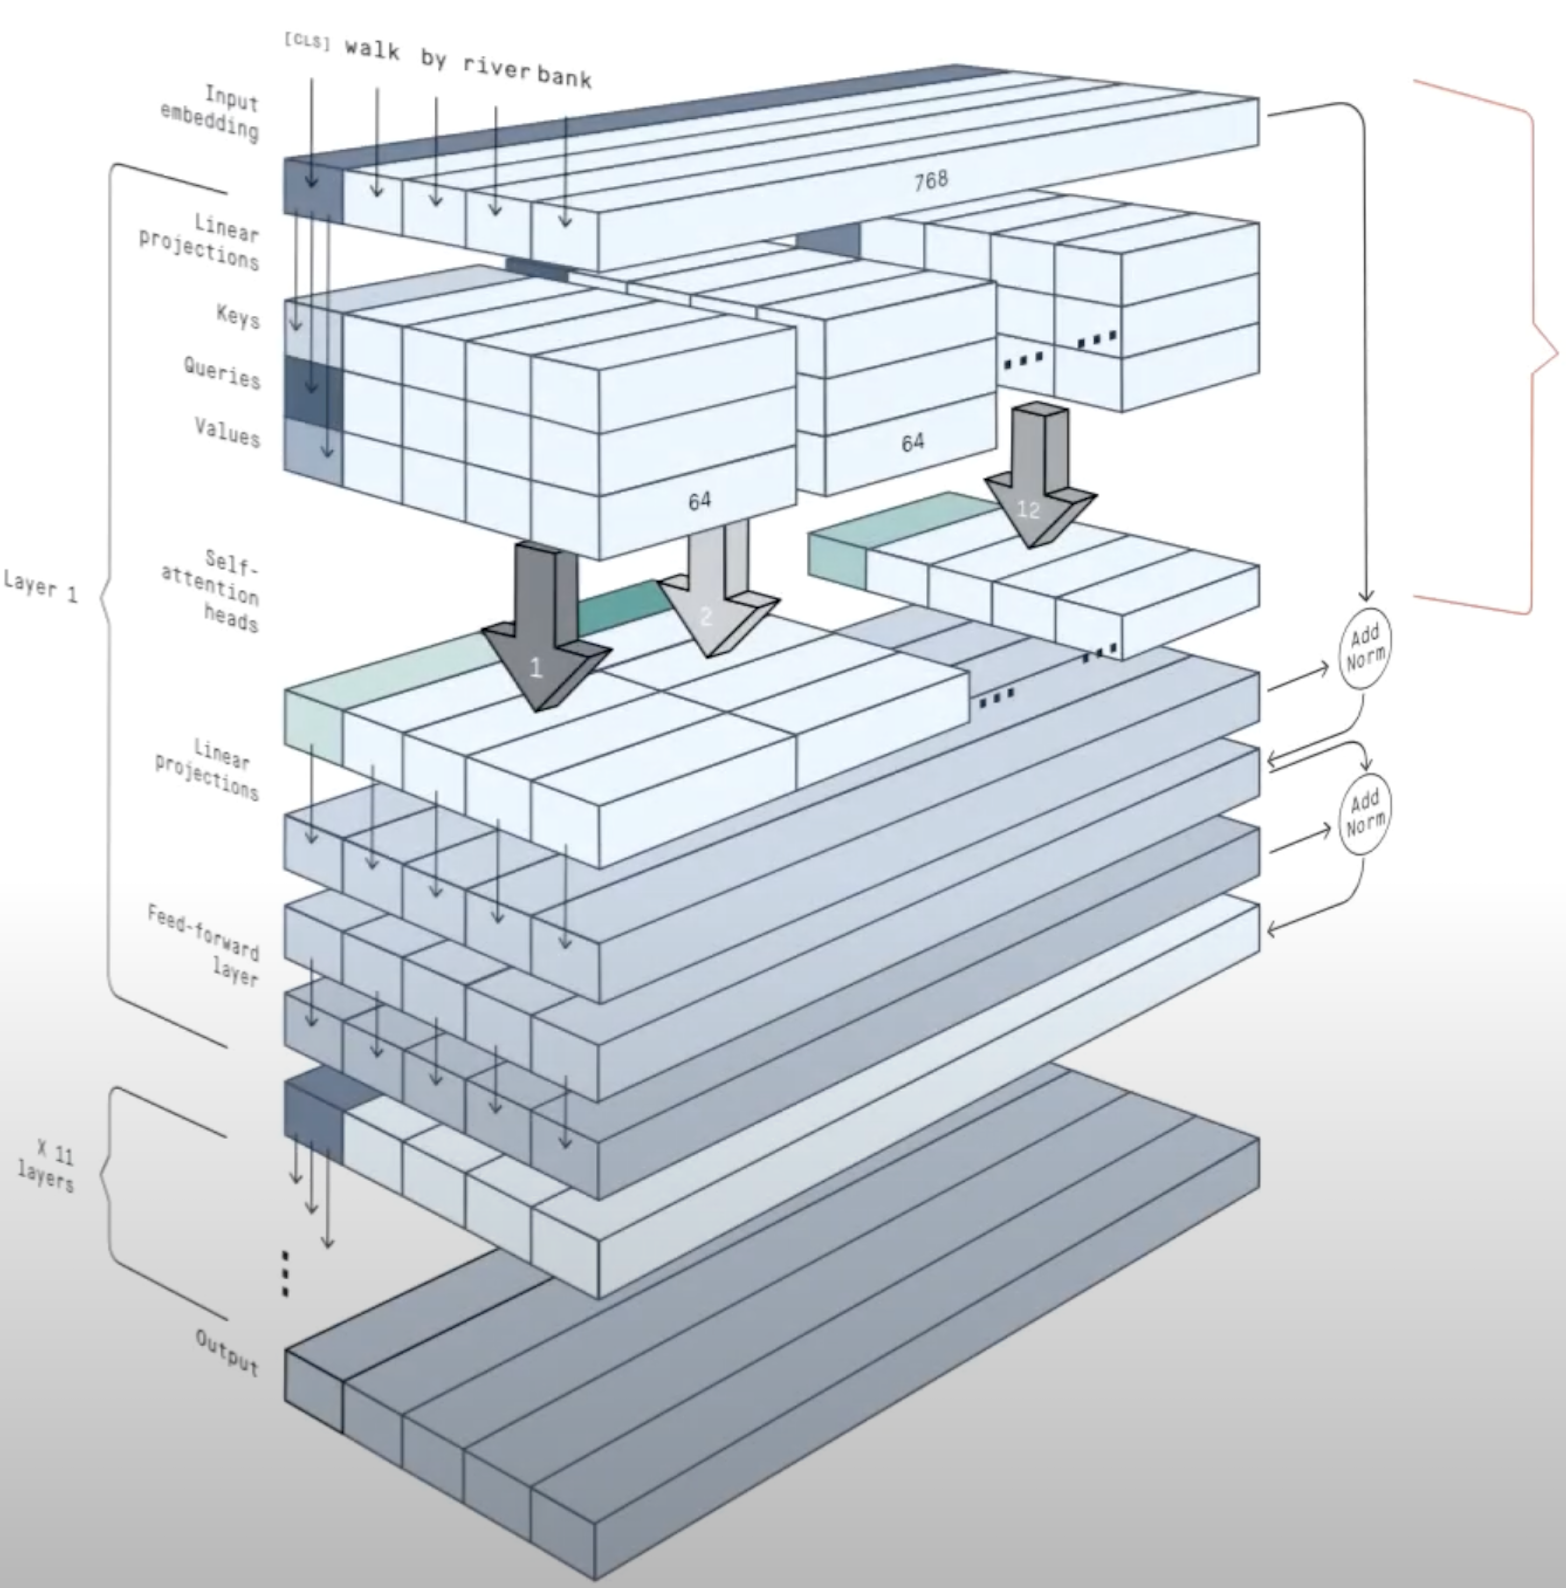
\includegraphics[scale=0.5]{static/BERT_visualization.png}
        \caption{\label{fig:BERT_visualization} Architektur des BERT Modells \cite{peltarion2020bert}}
    \end{center}
\end{figure}

\begin{figure}[htbp]
    \begin{center}
        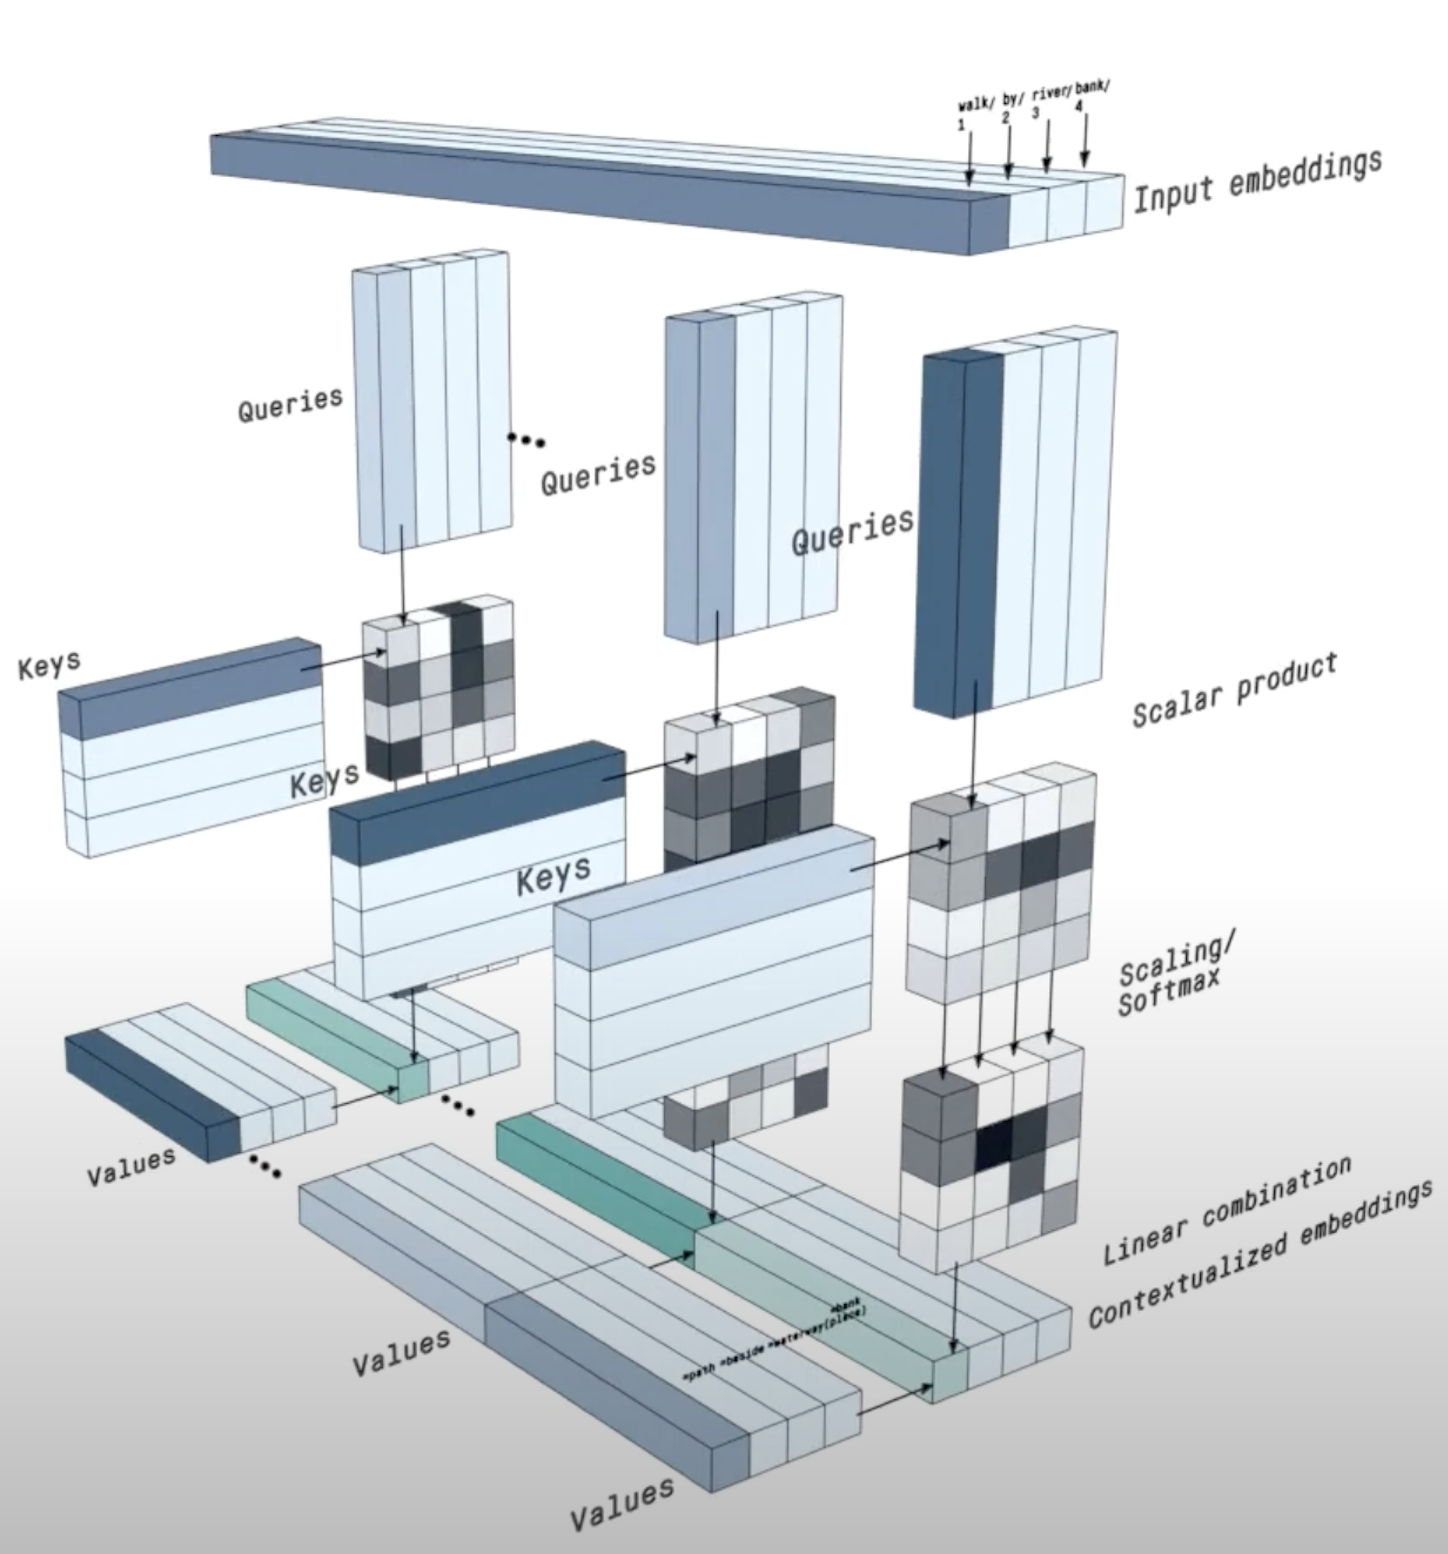
\includegraphics[scale=0.5]{static/multi-head_attention_visualization.png}
        \caption{\label{fig:multi_head_attention_visualization} Multi-Head Attention \cite{peltarion2020bert}}
    \end{center}
\end{figure}

\begin{figure}[htbp]
    \begin{center}
        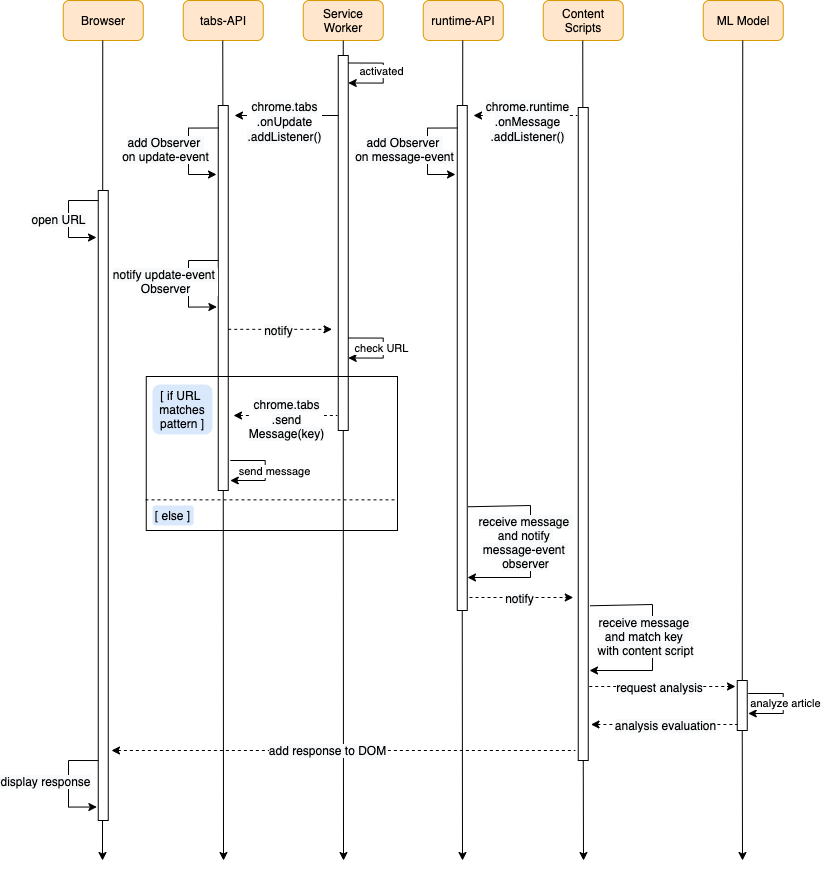
\includegraphics[scale=0.5]{diagrams/hauptkomponente_sequenzdiagramm.png}
        \caption{\label{fig:seq_hauptkomponente} Sequenzdiagramm Webagent}
    \end{center}
\end{figure}

\section{Tabellen}

\begin{table}[ht]
    \centering
    \renewcommand{\arraystretch}{1.3}
    \begin{tabular}{|p{2.5cm}|p{2.5cm}|p{2.5cm}|p{2.5cm}|p{2.5cm}|}
        \hline
        \textbf{Kriterium} & \textbf{Chrome Extension} & \textbf{Userscript (Tampermonkey)} & \textbf{Proxy-Server} & \textbf{Scraper + Plattform} \\
        \hline
        DOM-Zugriff beim Nutzer & Ja & Ja & Nein & Nein \\
        \hline
        Einbindung auf \texttt{bild.de} direkt & Ja & Ja & Ja (indirekt) & Nein \\
        \hline
        Installation durch Nutzer & Mittel & Einfach & Nicht erforderlich & Nicht erforderlich\\
        \hline
        Komplexität der Umsetzung & Mittel & Gering & Hoch & Mittel \\
        \hline
        Wartbarkeit \& Updates & Gut & Gut & Aufwändig & Mittel \\
        \hline
        Performance beim Nutzer & Hoch & Hoch & Hoch & Hoch \\
        \hline
        Skalierbarkeit & Hoch & Eingeschränkt & Mittel & Hoch \\
        \hline
        Für öffentliche Verbreitung geeignet & Ja & Eingeschränkt & Eingeschränkt & Ja \\
        \hline
        API-Nutzung zur Fake-Erkennung & Ja & Ja & Ja & Ja \\
        \hline
        Entwickler-kontrolle über UI & Hoch & Mittel & Hoch & Mittel \\
        \hline
    \end{tabular}
    \caption{Vergleich möglicher Technologien für den Webagenten}
    \label{table:technischeAnsaetze}
\end{table} %TODO: ChatGPT


\begin{sidewaystable}[htbp]
\centering
    \begin{tabular}{|p{3.5cm}|p{2.8cm}|p{2.8cm}|p{2.8cm}|p{2.8cm}|p{2.8cm}|}
        \hline
        \textbf{Merkmal} & \textbf{BERT Base} & \textbf{RoBERTa\newline Base} & \textbf{RoBERTa Large} & \textbf{XLM-RoBERTa Base} & \textbf{XLM-RoBERTa Large} \\
        \hline
        \textbf{Hidden Size} & 768 & 768 & 1024 & 768 & 1024 \\
        \hline
        \textbf{Anzahl Layer} & 12 & 12 & 24 & 12 & 24 \\
        \hline
        \textbf{Anzahl Attention Heads} & 12 & 12 & 16 & 12 & 16 \\
        \hline
        \textbf{Vocab Size} & 30,522 & 50,265 & 50,265 & 250,002 & 250,002 \\
        \hline
        \textbf{Spezialisiert auf} & Masked LM & Masked LM & Masked LM & Multilinguales Masked LM & Multilinguales Masked LM \\
        \hline
        \textbf{Sprachumfang} & Englisch & Englisch & Englisch & Multilingual & Multilingual \\
        \hline
    \end{tabular}
\caption{Vergleich der verschiedenen BERT- und RoBERTa-Modelle}
\label{tab:bert_models}
\end{sidewaystable}

